%%%%%%%%%%%%%%%%%%%%%%%%%%%%%%%%%%%%%%%%%%%%%%%%%%%%%%%%%%%%%%%
%
% Welcome to Overleaf --- just edit your LaTeX on the left,
% and we'll compile it for you on the right. If you open the
% 'Share' menu, you can invite other users to edit at the same
% time. See www.overleaf.com/learn for more info. Enjoy!
%
%%%%%%%%%%%%%%%%%%%%%%%%%%%%%%%%%%%%%%%%%%%%%%%%%%%%%%%%%%%%%%%

% Inbuilt themes in beamer
\documentclass{beamer}
\usepackage{setspace}
\usepackage{gensymb}
\singlespacing
\usepackage{amsmath}
\usepackage{bm}
\usepackage{cite}
\usepackage{cases}
\usepackage{subfig}
\usepackage{longtable}
\usepackage{multirow}
\usepackage{verbatim}
\usepackage{hyperref}
\usepackage{listings}
\usepackage{color}    
\usepackage{array}    
\usepackage{longtable}
\usepackage{calc}     
\usepackage{listings}
\usepackage{graphicx}
\usepackage{multirow} 
\usepackage{hhline}   
\usepackage{ifthen}  
\usepackage{tikz}
\usetikzlibrary{positioning,shapes.geometric,arrows.meta} % positioning is required
\tikzset{
  block/.style = {rectangle, rounded corners,
                  minimum width=4cm, minimum height=1cm,
                  draw=black, fill=gray!20, align=center},
  arrow/.style = {very thick, -{Stealth[length=3mm,width=2mm]}}
}
\usepackage{circuitikz}
\usetikzlibrary{shapes.geometric, arrows}
\DeclareMathOperator*{\Res}{Res}

% correct bad hyphenation here
\hyphenation{op-tical net-works semi-conduc-tor}
\def\inputGnumericTable{}                                 %%

\lstset{
%language=C,
frame=single, 
breaklines=true,
columns=fullflexible
}
%\lstset{
%language=tex,
%frame=single, 
%breaklines=true
%}
\hypersetup{
    colorlinks=true,
    linkcolor=black,
    urlcolor=blue,
}
\usetheme{CambridgeUS}

\DeclareMathOperator*{\argmax}{arg\,max}
\DeclareMathOperator*{\argmin}{arg\,min}
\newtheorem{proposition}{Proposition}[section]
\newcommand{\BEQA}{\begin{eqnarray}}
\newcommand{\EEQA}{\end{eqnarray}}
\newcommand{\define}{\stackrel{\triangle}{=}}
\bibliographystyle{IEEEtran}
\providecommand{\mbf}{\mathbf}
\providecommand{\pr}[1]{\ensuremath{\Pr\left(#1\right)}}
\providecommand{\qfunc}[1]{\ensuremath{Q\left(#1\right)}}
\providecommand{\sbrak}[1]{\ensuremath{{}\left[#1\right]}}
\providecommand{\lsbrak}[1]{\ensuremath{{}\left[#1\right.}}
\providecommand{\rsbrak}[1]{\ensuremath{{}\left.#1\right]}}
\providecommand{\brak}[1]{\ensuremath{\left(#1\right)}}
\providecommand{\lbrak}[1]{\ensuremath{\left(#1\right.}}
\providecommand{\rbrak}[1]{\ensuremath{\left.#1\right)}}
\providecommand{\cbrak}[1]{\ensuremath{\left\{#1\right\}}}
\providecommand{\lcbrak}[1]{\ensuremath{\left\{#1\right.}}
\providecommand{\rcbrak}[1]{\ensuremath{\left.#1\right\}}}
\theoremstyle{remark}
\newtheorem{rem}{Remark}
\newcommand{\sgn}{\mathop{\mathrm{sgn}}}
\providecommand{\abs}[1]{\left\vert#1\right\vert}
\providecommand{\res}[1]{\Res\displaylimits_{#1}} 
\providecommand{\norm}[1]{\left\lVert#1\right\rVert}
\providecommand{\mtx}[1]{\mathbf{#1}}
\providecommand{\mean}[1]{\mathbb{E}\left[ #1 \right]}   
\providecommand{\fourier}{\overset{\mathcal{F}}{ \rightleftharpoons}}
\providecommand{\system}[1]{\overset{\mathcal{#1}}{ \longleftrightarrow}}
\newcommand{\cosec}{\,\text{cosec}\,}
\providecommand{\dec}[2]{\ensuremath{\overset{#1}{\underset{#2}{\gtrless}}}}
\newcommand{\myvec}[1]{\ensuremath{\begin{pmatrix}#1\end{pmatrix}}}
\newcommand{\mydet}[1]{\ensuremath{\begin{vmatrix}#1\end{vmatrix}}}
\renewcommand{\vec}[1]{\mathbf{\boldsymbol{#1}}}
% Theme choice:
\newcounter{saveenumi}
\newcommand{\seti}{\setcounter{saveenumi}{\value{enumi}}}
\newcommand{\conti}{\setcounter{enumi}{\value{saveenumi}}}

\resetcounteronoverlays{saveenumi}
% Title page details: 
\title{Calculator Implementation on Vaman FPGA}  
\author{Siddhant Yellanki}
\begin{document}

% Title page frame
\begin{frame}
    \titlepage 
\end{frame}

% Remove logo from the next slides
\logo{}

% Outline frame
\begin{frame}{Outline}
    \tableofcontents
\end{frame}

% Lists frame
\section{Introduction}
\begin{frame}{Introduction}
    \begin{enumerate}
        \item This paper presents the design and implementation of a scientific calculator on a Vaman FPGA, using a synthesizable Verilog library for fixed-point arithmetic and elementary functions in the Q16.47 format.
        \item The system includes modules for addition, multiplication, division, comparison, and transcendental functions (sine, cosine, tangent, exponential), as well as a converter for displaying fixed-point results as ASCII characters.
        \item The calculator provides a user interface for entering numbers and operations, and displays results in human-readable decimal format.
        \item It uses numerical methods such as Euler's method and Newton-Raphson iterations to calculate the values of the transcendental functions up to an accuracy of 4 digits.
    \end{enumerate}
\end{frame}

\section{System Overview}
\begin{frame}{System Overview}
    The calculator system consists of the following components:
    \begin{itemize}
        \item User input interface (5 x 5 Button Array)
        \item Arithmetic and function modules (Q16.47 math library)
        \item ASCII conversion for display
        \item Output interface (16x2 LCD Display)
    \end{itemize}
    The entire design is implemented in Verilog and targeted for FPGA synthesis.
\end{frame}

\begin{frame}{System Overview}
\centering
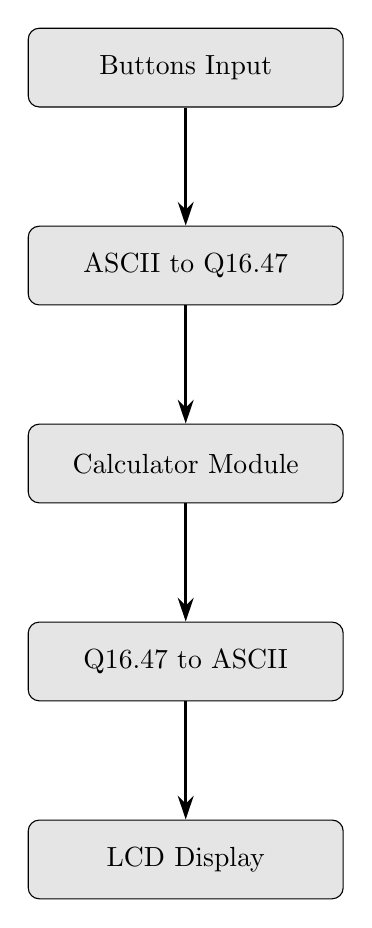
\begin{tikzpicture}[node distance=1.5cm]

\node (input)   [block]                {Buttons Input};
\node (ascii2q) [block, below=of input]   {ASCII to Q16.47};
\node (calc)    [block, below=of ascii2q] {Calculator Module};
\node (q2ascii) [block, below=of calc]    {Q16.47 to ASCII};
\node (lcd)     [block, below=of q2ascii] {LCD Display};

\draw[arrow] (input) -- (ascii2q);
\draw[arrow] (ascii2q) -- (calc);
\draw[arrow] (calc) -- (q2ascii);
\draw[arrow] (q2ascii) -- (lcd);

\end{tikzpicture}
\end{frame}

\begin{frame}{Components}
    \centering
    \begin{tabular}{|l|c|c|}
    \hline
    Component & Value & Quantity\\
    \hline
    Vaman Board & & 1\\
    \hline
    USB-UART & & 1\\
    \hline
    16x2 LCD Display & & 1\\
    \hline
    Push Buttons & & 25\\
    \hline
    Slide Switch&  & 1\\
    \hline
    Jumper Wires & F-M & 30\\
    \hline
    Wires &  & \\
    \hline
    Breadboard & & 2\\
    \hline
    \end{tabular}\\
    \
    \centerline{Table 1.0}
\end{frame}

\section{Circuit Connections}
\subsection{Input Keyboard Connections}
\begin{frame}{Input Keyboard Connections}
    \centering
\begin{tabular}{|c|c|c|}
\hline
BUTTON & VAMAN BOARD & Name\\
\hline
Button 1 & PYGMY 1 & Num 0\\
\hline
Button 2 & PYGMY 2 & Num 1\\
\hline
Button 3 & PYGMY 3 & Num 2\\
\hline
Button 4 & PYGMY 4 & Num 3\\
\hline
Button 5 & PYGMY 5 & Num 4\\
\hline
Button 6 & PYGMY 6 & Num 5\\
\hline
Button 7& PYGMY 7& Num 6\\
\hline
Button 8 & PYGMY 8 & Num 7\\
\hline
Button 9 & PYGMY 9 & Num 8\\
\hline
Button 10 & PYGMY 10 & Num 9\\
\hline
\end{tabular}\\
\end{frame}

\begin{frame}{Input Keyboard Connections}
    \centering
    \begin{tabular}{|c|c|c|}
        \hline
        Button 11 & PYGMY 11& Plus \\
        \hline
        Button 12 & PYGMY 12 & Minus\\
        \hline
        Button 13 & PYGMY 13 & Multiply\\
        \hline
        Button 14 & PYGMY 14 & Divide\\
        \hline
        Button 15 & PYGMY 15 & Sin\\
        \hline
        Button 16 & PYGMY 16 & Cos\\
        \hline
        Button 17 & PYGMY 17 & Tan\\
        \hline
        Button 18 & PYGMY 18 & Exp\\
        \hline
        Button 19 & PYGMY 19 & Enter\\
        \hline
        Button 20 & PYGMY 20 & Decimal\\
        \hline
        Button 21 & PYGMY 21 & Reset\\
        \hline
        Toggle & PYGMY 22 & Function Toggle\\
        \hline
    \end{tabular}
    \
    \centerline{Table 2.0}
\end{frame}

\subsection{LCD Connections}
\begin{frame}{LCD Connections}
    \raggedright
    Make the Circuit Connections as per the table below.\\
    \vspace{0.25cm}
    \centering
        \begin{tabular}{|l|c|l|l|}
            \hline
            \textbf{Vaman} & \textbf{LCD} & \textbf{LCD Name} & \textbf{LCD Description} \\
            \hline
            GND & 1 & GND & \\
            \hline
            5V & 2 & Vcc & \\
            \hline
            GND & 3 & Vee & Contrast \\
            \hline
            PYGMY 23 & 4 & RS & Register Select \\
            \hline
            GND & 5 & R/W & Read/Write \\
            \hline
            PYGMY 24 & 6 & EN & Enable \\
            \hline
            PYGMY 25 & 11 & DB4 & Serial Connection \\
            \hline
            PYGMY 26 & 12 & DB5 & Serial Connection \\
            \hline
            PYGMY 27 & 13 & DB6 & Serial Connection \\
            \hline
            PYGMY 28 & 14 & DB7 & Serial Connection \\
            \hline
            5V & 15 & LED+ & Backlight \\
            \hline
            GND & 16 & LED- & Backlight \\
            \hline
        \end{tabular}
    \\
    \
    \centerline{Table 3.0}
\end{frame}

\section{Q16.47 Fixed-Point Format}
\begin{frame}{Q16.47 Fixed-Point Format}
    A Q16.47 fixed-point number is a 64-bit signed value:
\begin{itemize}
    \item \textbf{Bit 63:} Sign bit (0 for positive, 1 for negative)
    \item \textbf{Bits 62:47:} Integer part (16 bits)
    \item \textbf{Bits 46:0:} Fractional part (47 bits)
\end{itemize}
The value is:
\begin{equation}
    \text{Value} = (-1)^{\text{sign}} \times \left(\text{Integer Part} + \frac{\text{Fractional Part}}{2^{47}}\right)
\end{equation}
The reason behind this format rather than using the industry standard IEEE-754 Single Precision Floating Point format, is due to the ease of implementing, fast calculation and low error accumulation rate. 
\end{frame}

\subsection{Q16.47 Fixed Point Format}
\begin{frame}{Q16.47 Fixed Point Format}
    \begin{enumerate}
        \item Connections to floating point to fixed point\\
        Fixed point is very simple as it is simply just shifting of bits. So to convert to fixed point,
    \begin{align}
        Float = \frac{Fixed}{2^{47}}
    \end{align}
    \item Conversion to Fixed Point from Floating Point
    Similarly, compared to converting to fixed point,
\begin{align}
    Fixed = {Float}\times{2^{47}}
\end{align}
\item Range of the calculator
Since, we have 63 bits of working integers, the range is $\pm 2^{63-47}$ or -65536 to 65536. In the code, 65536 is defined as infinity.
    \end{enumerate}
\end{frame}

\section{Arithmetic Modules}
\begin{frame}{Arithmetic Modules}
\begin{enumerate}
    \item Adder
    \item Multiplier
    \item Divider
    \item Comparison
\end{enumerate}
\end{frame}

\subsection{Adder}
\begin{frame}{Adder}
    The adder module performs signed addition of two Q16.47 numbers.
This module is fully synthesizable and handles two's complement arithmetic.

\textbf{Limitations and Edge Cases:}
\begin{itemize}
    \item The output saturates to the maximum if the sum exceeds the representable range of Q16.47 (i.e., overflow/underflow is possible but not flagged).
\end{itemize}
\end{frame}

\subsection{Multiplier}
\begin{frame}{Multiplier}
    The multiplier module multiplies two Q16.47 numbers and aligns the result using bit shifting.
This implementation uses two's complement arithmetic and checks for overflow.

\textbf{Limitations and Edge Cases:}
\begin{itemize}
    \item If the product exceeds the Q16.47 representable range, the overflow flag is set.
    \item Overflow does not saturate the output; the result wraps around as per two's complement arithmetic.
    \item Multiplying by zero always yields zero.
    \item Multiplying the largest positive and negative values can result in overflow.
    \end{itemize}
\end{frame}

\subsection{Divider}
\begin{frame}{Divider}
   The divider module implements non-restoring division using shift and subtract.
The divider supports signed division and overflow detection.

\textbf{Limitations and Edge Cases:}
\begin{itemize}
    \item Division by zero: If the divisor is zero, the overflow flag is set, and the quotient output is undefined (may be set to the maximum positive or negative value, depending on implementation).
    \item Division overflow: If the result exceeds the Q16.47 range, the overflow flag is set.
    \item Division of zero by any nonzero number yields the maximum possible number 65536.
\end{itemize}
\end{frame}

\begin{frame}{Comparison}
The fixedCompare module compares the absolute values of two Q16.47 numbers. This is mainly used in the iterative approach of the transcendental functions, to compare between the current iteration and the maximum iteration.
\end{frame}

\section{Transcendental Function Modules}
\begin{frame}{Transcendental Function Modules}
    The transcendental functions are implemented using iterative or difference-equation-based numerical methods, leveraging the arithmetic modules. Below, we provide not only the update equations, but also the underlying derivations for commonly used methods such as Forward Euler, Double Euler (Leapfrog), and RK2.
\end{frame}

\subsection{sin(x): Double Euler Method}
\begin{frame}{sin(x): Double Euler Method}
    To compute \(\sin(x)\), recognize the second-order ordinary differential equation:
\begin{align*}
	\frac{d^2 y(x)}{dx^2} &= -y(x)
\end{align*}
where \(y(x) = \sin(x)\) and \(\frac{d^2 \sin(x)}{dx^2} = -\sin(x)\).

Approximating the second derivative at a point \(x_n\) using the centered finite difference:
\begin{align*}
	\frac{y_{n+1} - 2y_n + y_{n-1}}{h^2} &\approx \frac{d^2 y}{dx^2}\bigg|_{x_n} 
\end{align*}
Substituting into the ODE:
\end{frame}

\begin{frame}{sin(x):Double Euler Method}
    \begin{align*}
	\frac{y_{n+1} - 2y_n + y_{n-1}}{h^2} = -y_n \\
	\Rightarrow y_{n+1} = 2y_n - y_{n-1} - h^2 y_n
\end{align*}
Initialization: 
\[
y_0 = 0, \quad y_1 = h, \quad h = \frac{1}{2^{16}}
\]
or, in fixed point: $ y_0 = 64'd0, y_1 = 64'h0000000080000000$\\ 
,$h = 64'h0000000080000000 $.

For improved fixed-point precision, \(h\) may be chosen as \(h = \frac{1}{2^{15}}\), meaning \(h^2 = \frac{1}{2^{30}}\), which offers sufficient resolution for the system.
\end{frame}

\subsection{cos(x):Double Euler Method(different initial Condition)}
\begin{frame}{cos(x):Double Euler Method(different initial Condition)}
    Using the same update equation as for \(\sin(x)\), but initializing to match the series expansion for \(\cos(x)\):
\[
y_0 = 1, \quad y_1 = 0.999, \quad h = \frac{1}{2^{16}}
\]
or in fixed point:
$
y_0 = 64'h0000800000000000, y_1 = 64'h00007FFFFFFFC000, h = 64'h0000000080000000
$
\end{frame}

\subsection{tan(x): Forward Euler Method}
\begin{frame}{tan(x): Forward Euler Method}
    The governing ODE for the tangent is:
\[
\frac{dy}{dx} = 1 + y^2
\]
Applying the (explicit) forward Euler method, where the derivative is approximated as:
\[
\frac{y_{n+1} - y_n}{h} \approx f(y_n, x_n)
\]
leads to:
\begin{align*}
	y_{n+1} = y_n + (1 + y_n^2)h
\end{align*}
with initial conditions \( y_0 = 0,\, h = \frac{1}{2^{16}} \), or in fixed point, \( y_0 = 64'd0,\, h = 64'h0000000080000000 \).
\end{frame}

\subsection{exp(x): RK2 (Midpoint Method)}
\begin{frame}{exp(x): RK2 (Midpoint Method)}
For exponentials, the differential equation is:
\[
\frac{dy}{dx} = y
\]
To solve with second-order accuracy, the RK2 (midpoint) method is:
\begin{align*}
	k_1 &= h f(x_n, y_n) = h y_n \\
	k_2 &= h f\left(x_n + \frac{h}{2}, \, y_n + \frac{k_1}{2}\right) = h(y_n + \frac{k_1}{2}) \\
	y_{n+1} &= y_n + \frac{1}{2}(k_1 + k_2)
\end{align*}
\end{frame}

\begin{frame}{exp(x): RK2 (Midpoint Method)}
This is derived by taking an Euler step to the midpoint, evaluating the slope there, and then updating from the average of the starting and midpoint slopes.

\textbf{Initial conditions}: \( y_0 = 1,\, x_0 = 0,\, h = 0.01 \). \\
In fixed point: \( x_0 = 64'd0,\, y_0 = 64'h0000800000000000,\, h = 64'h0000000080000000 \).
\end{frame}

\subsection*{Summary Table of Methods}
\begin{frame}{Summary Table of Methods}
\begin{table}[ht]
\centering
\begin{tabular}{|c|c|c|l|}
\hline
Function & ODE & Method & Iteration Formula \\
\hline
$\sin(x)$    & $y''(x) = -y(x)$  & Double Euler & $y_{n+1} = 2y_n - y_{n-1} - h^2 y_n$ \\
$\cos(x)$    & $y''(x) = -y(x)$  & Double Euler & $y_{n+1} = 2y_n - y_{n-1} - h^2 y_n$ \\
$\tan(x)$    & $y'(x) = 1+y^2$   & Euler        & $y_{n+1} = y_n + (1 + y_n^2) h$ \\
$\exp(x)$    & $y'(x) = y(x)$    & RK2          & $\begin{aligned}
k_1 &= h y_n \\
k_2 &= h (y_n + \frac{k_1}{2})\\
y_{n+1} &= y_n + \frac{k_1 + k_2}{2}
\end{aligned}$ \\
\hline
\end{tabular}
\end{table}
\end{frame}

\section{Fixed-Point to ASCII (\texttt{fta}) and ASCII to Fixed-Point (\texttt{atf}) Modules}
\subsection{The \texttt{fta} Module: Fixed-Point to ASCII Conversion}
\begin{frame}{The \texttt{fta} Module: Fixed-Point to ASCII Conversion}
The \texttt{fta} module converts a fixed-point binary number into its human-readable ASCII decimal representation. This is essential for displaying calculation results on an LCD or other character-based interfaces.

\begin{itemize}
    \item \textbf{Input:} A fixed-point number \texttt{value} of width $N$ (e.g., 64 bits), with $Q$ bits for the fractional part.
    \item \textbf{Output:} An array of ASCII characters (\texttt{ascii\_array}) representing the signed decimal value, e.g., ``-12.3456''.
\end{itemize}
\end{frame}

\begin{frame}{The \texttt{fta} Module: Fixed-Point to ASCII Conversion}
    The conversion process:
\begin{enumerate}
    \item \textbf{Sign Extraction:} The sign bit is checked. If negative, the value is negated and a ``-'' is added to the ASCII output.
    \item \textbf{Integer Part:} The integer portion is extracted by right-shifting the value by $Q$ bits. This integer is then converted to ASCII digits by repeated division and modulo by 10.
    \item \textbf{Decimal Point:} A ``.'' character is inserted after the integer digits.
    \item \textbf{Fractional Part:} The fractional portion (the lower $Q$ bits) is scaled up (multiplied by $10^n$ for $n$ decimal digits) and right-shifted by $Q$ to get the decimal representation, which is then converted to ASCII digits.
    \item \textbf{Output Formatting:} The ASCII characters are stored in the output array, padded with spaces if necessary.
\end{enumerate}
\end{frame}

\subsection{The \texttt{atf} Module: ASCII to Fixed-Point Conversion}
\begin{frame}{The \texttt{atf} Module: ASCII to Fixed-Point Conversion}
The \texttt{atf} module performs the reverse operation: converting an ASCII string representing a decimal number into a fixed-point binary value.

\begin{itemize}
    \item \textbf{Input:} An array of ASCII characters (\texttt{ascii\_array}) representing a number, e.g., ``-12.3456''.
    \item \textbf{Output:} A fixed-point number \texttt{value} of width $N$ and $Q$ fractional bits.
\end{itemize}
\end{frame}

\begin{frame}{The \texttt{fta} Module: Fixed-Point to ASCII Conversion}
The conversion process:
\begin{enumerate}
    \item \textbf{Sign Detection:} Checks for a leading ``-'' character to determine if the result should be negative.
    \item \textbf{Integer Part Parsing:} Reads ASCII digits before the decimal point, accumulating the integer value.
    \item \textbf{Fractional Part Parsing:} After the decimal point, reads ASCII digits, accumulating the fractional value and counting the number of digits.
    \item \textbf{Fixed-Point Assembly:} The integer part is left-shifted by $Q$ bits. The fractional part is scaled to fit into $Q$ bits (i.e., \texttt{frac\_accum * 2\^Q / 10\^d}, where $d$ is the number of fractional digits).
    \item \textbf{Sign Application:} If the input was negative, the two's complement is applied to the result.
\end{enumerate}
\end{frame}

\section{Performance}
\begin{frame}{Performance}
All modules use synthesizable constructs:
\begin{itemize}
    \item \textbf{Combinational logic:} Implemented with \texttt{always @(*)}.
    \item \textbf{Static arrays and loops:} Loops are unrolled by synthesis tools.
    \item \textbf{Arithmetic:} Addition, multiplication, and division are synthesizable, though division by 10 (for ASCII conversion) may be resource-intensive.
    \item \textbf{Parameterization:} All modules are parameterized for flexibility.
\end{itemize}
Overflow detection and sign handling are included throughout.
\end{frame}

\section{Accuracy}
\begin{frame}{Accuracy}
To measure the accuracy of the calculator, we will compare it with C standard results.
\begin{enumerate}
    \item Sin(x)
    \item cos(x)
    \item tan(x)
    \item exp(x)
\end{enumerate}
\end{frame}

\subsection{Sin(x)}
\begin{frame}{Sin(x)}
    \begin{table}[h!]
\centering
\begin{tabular}{|c|c|c|}
\hline
$x$ & $sinFixed(x)$ & $sin(x)$ \\
\hline
1    & 0.8414792291   & 0.8414709848 \\
2    & 0.9092910765   & 0.9092974268 \\
1.57 & 0.9999997006   & 0.9999996829 \\
\hline
\end{tabular}
\end{table}
\end{frame}

\subsection{Cos(x)}
\begin{frame}{Cos(x)}
\begin{table}[h!]
\centering
\begin{tabular}{|c|c|c|}
\hline
$x$ & $cosFixed(x)$ & $cos(x)$ \\
\hline
1    & 0.5402894659    & 0.5403023059 \\
2    & -0.4161607117   & -0.4161468365 \\
1.57 & 0.0007737434    & 0.0007963267 \\
\hline
\end{tabular}
\end{table}
\end{frame}

\subsection{Tan(x)}
\begin{frame}{Tan(x)}
\begin{table}[h!]
\centering
\begin{tabular}{|c|c|c|}
\hline
$x$ & $tanFixed(x)$ & $tan(x)$ \\
\hline
1    & 1.5573755479   & 1.5574077247 \\
1.57 & 1186.2765882125 & 1255.7655915008 \\
\hline
\end{tabular}
\end{table}    
\end{frame}

\subsection{Exp(x)}
\begin{frame}{Exp(x)}
\begin{table}[h!]
\centering
\begin{tabular}{|c|c|c|}
\hline
$x$ & $expFixed(x)$ & $exp(x)$ \\
\hline
1   & 2.7182714591   & 2.7182818285 \\
1.5 & 4.4816634261   & 4.4816890703 \\
3.2 & 24.5325301975  & 24.5325301971 \\
\hline
\end{tabular}
\end{table}
\end{frame}

\section{Execution}
\begin{frame}[fragile]{Execution}
\begin{itemize}
    \item Download the repository
    \begin{verbatim}
git clone https://github.com/ysiddhanth/vaman.git
cd vaman
\end{verbatim}

    \item Locate the folder codes, in the Calculator folder.
    \begin{verbatim}
cd Calculator/codes
\end{verbatim}

    \item Generate the .bin file
    \begin{verbatim}
ql_symbiflow -compile -src . -d ql-eos-s3 -P pu64 -t main -v main.v -p quickfeather.pcf -dump binary
\end{verbatim}

    \item Dump .bin files on the Vaman FPGA
    \begin{verbatim}
sudo python3 <tinyfpga uploader> --port /dev/ttyACM0  --appfpga main.bin --mode fpga --reset
\end{verbatim}
\end{itemize}
\end{frame}
\section{Hardware Built}
\begin{frame}{Hardware Built}
    \begin{itemize}
    \item Connect the LCD Display and the buttons to the breadboard and make the connections to the fpga according to the above tables.
\end{itemize}
\centering
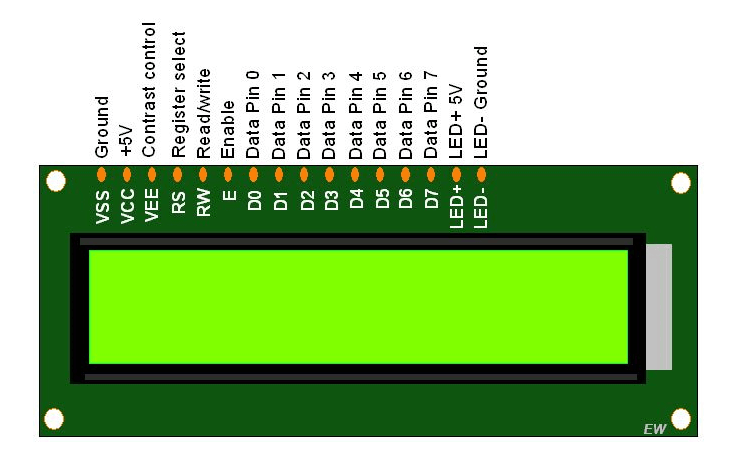
\includegraphics[width=0.5\textwidth]{figs/lcd.png}
\centerline{Figure 1 -  LCD Pinout}
\end{frame}
\begin{frame}{Hardware Built}
\centering
    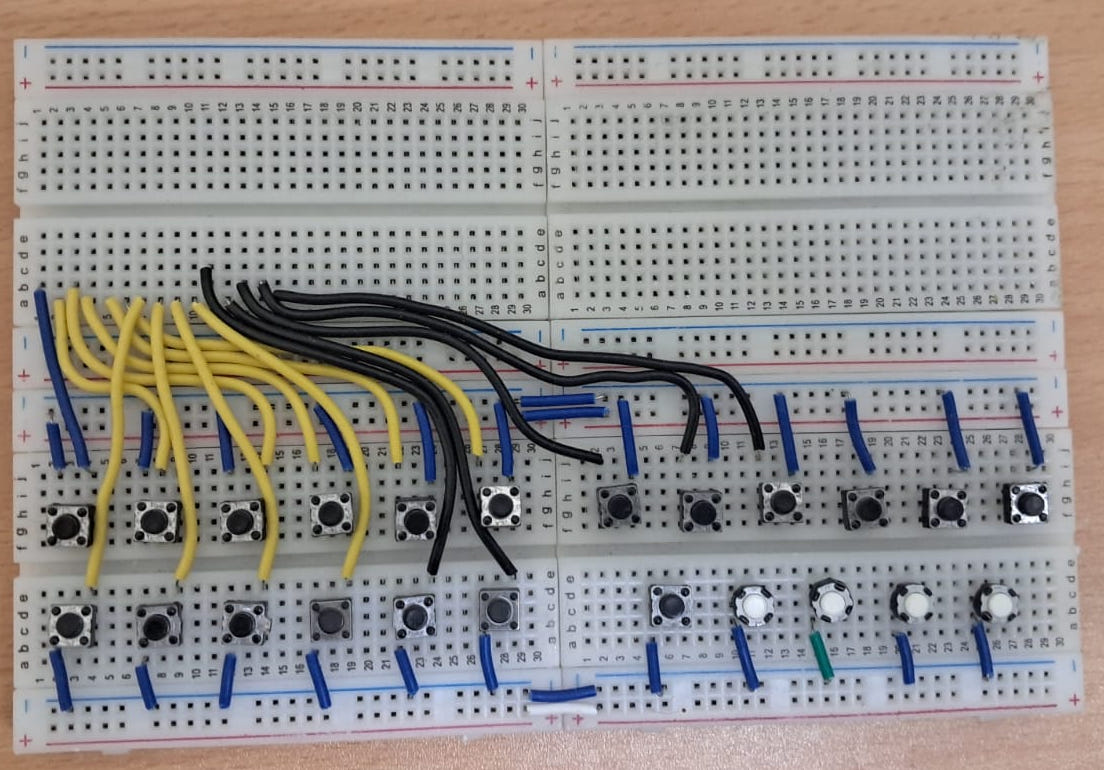
\includegraphics[width=0.5\textwidth]{figs/buttons.jpeg}
\centerline{Figure 2 -  Button Arrangement}
\end{frame}
\begin{frame}{Hardware Built}
\centering
    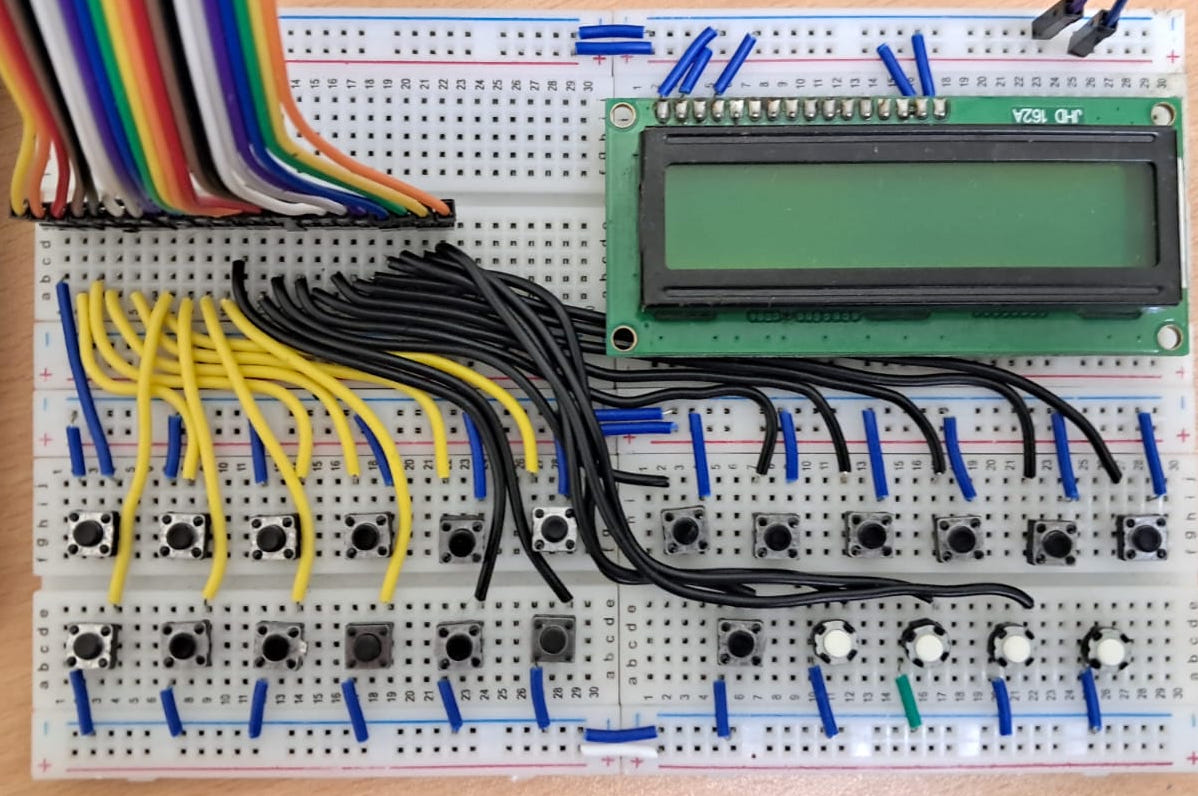
\includegraphics[width=0.5\textwidth]{figs/final.jpeg}
\centerline{Figure 3 -  The calculator}
\end{frame}

\end{document}
